% Options for packages loaded elsewhere
\PassOptionsToPackage{unicode}{hyperref}
\PassOptionsToPackage{hyphens}{url}
%
\documentclass[
]{report}
\usepackage{lmodern}
\usepackage{amssymb,amsmath}
\usepackage{ifxetex,ifluatex}
\ifnum 0\ifxetex 1\fi\ifluatex 1\fi=0 % if pdftex
  \usepackage[T1]{fontenc}
  \usepackage[utf8]{inputenc}
  \usepackage{textcomp} % provide euro and other symbols
\else % if luatex or xetex
  \usepackage{unicode-math}
  \defaultfontfeatures{Scale=MatchLowercase}
  \defaultfontfeatures[\rmfamily]{Ligatures=TeX,Scale=1}
\fi
% Use upquote if available, for straight quotes in verbatim environments
\IfFileExists{upquote.sty}{\usepackage{upquote}}{}
\IfFileExists{microtype.sty}{% use microtype if available
  \usepackage[]{microtype}
  \UseMicrotypeSet[protrusion]{basicmath} % disable protrusion for tt fonts
}{}
\makeatletter
\@ifundefined{KOMAClassName}{% if non-KOMA class
  \IfFileExists{parskip.sty}{%
    \usepackage{parskip}
  }{% else
    \setlength{\parindent}{0pt}
    \setlength{\parskip}{6pt plus 2pt minus 1pt}}
}{% if KOMA class
  \KOMAoptions{parskip=half}}
\makeatother
\usepackage{xcolor}
\IfFileExists{xurl.sty}{\usepackage{xurl}}{} % add URL line breaks if available
\IfFileExists{bookmark.sty}{\usepackage{bookmark}}{\usepackage{hyperref}}
\hypersetup{
  pdfauthor={Johannes Altmanninger},
  hidelinks,
  pdfcreator={LaTeX via pandoc}}
\urlstyle{same} % disable monospaced font for URLs
\usepackage{graphicx,grffile}
\makeatletter
\def\maxwidth{\ifdim\Gin@nat@width>\linewidth\linewidth\else\Gin@nat@width\fi}
\def\maxheight{\ifdim\Gin@nat@height>\textheight\textheight\else\Gin@nat@height\fi}
\makeatother
% Scale images if necessary, so that they will not overflow the page
% margins by default, and it is still possible to overwrite the defaults
% using explicit options in \includegraphics[width, height, ...]{}
\setkeys{Gin}{width=\maxwidth,height=\maxheight,keepaspectratio}
% Set default figure placement to htbp
\makeatletter
\def\fps@figure{htbp}
\makeatother
\setlength{\emergencystretch}{3em} % prevent overfull lines
\providecommand{\tightlist}{%
  \setlength{\itemsep}{0pt}\setlength{\parskip}{0pt}}
\setcounter{secnumdepth}{-\maxdimen} % remove section numbering
\usepackage{todonotes}
\usepackage{longtable}
\usepackage{booktabs}
\title{
    DRAT Proofs Without Deletions of \\ Unique Reason Clauses \\
    \&\\
    Complete and Efficient \\ DRAT Proof Checking
}

\author{Johannes Altmanninger}
\date{\today}

\begin{document}

\maketitle

\textbf{Abstract:} Clausal proof format DRAT is the de facto standard
way to certify SAT solvers' unsatisfiability results. State-of-the-art
DRAT proof checkers ignore deletions of unit clauses, which means that
they are checking against a proof system that differs from the
specification of DRAT and they may not be able to verify inprocessing
techniques that use unit deletions. State-of-the-art SAT solvers produce
proofs that are accepted by DRAT checkers, but are incorrect under the
DRAT specification, because they contain spurious deletions of reason
clauses. We present patches for award-winning SAT solvers to produce
proofs without those deletions that are thus correct with respect to the
specification. Performing unit deletions in a proof checker can be
computationally expensive. We implemented the first competitive checker
that honors unit deletions and provide experimental results suggesting
that, on average, checking costs are the same as when not applying unit
deletions. As it is also expensive to determine the (in-)correctness of
a proof, we present the SICK format which describes small and
efficiently checkable certificates of the incorrectness of a DRAT proof.
This increases trust in incorrectness results and can be useful when
debugging solvers and checkers.

\tableofcontents

\hypertarget{introduction}{%
\chapter{1. Introduction}\label{introduction}}

Over the past decades, there has been significant progress in SAT
solving technology. SAT solvers have had documented bugs
{[}\protect\hyperlink{ref-BrummayerBiere-SMT09}{1}{]}
{[}\protect\hyperlink{ref-DBLP:confux2fsatux2fBrummayerLB10}{2}{]}. To
detect incorrect results, there are \emph{checker} programs that
\emph{verify} a solver's result based on a witness given by the solver.
Satisfiability witnesses, or \emph{models} can be checked in linear
time. Unsatisfiability witnesses, or \emph{proofs} of unsatisfiability
on the other hand can be much more costly to check.

A SAT solver operates on a formula that acts as knowledge base. It
contains constraints that are called clauses. Starting from the input
formula, clauses are added and deleted by the solver. In SAT
competitions, solvers are required to give proofs of unsatisfiability in
the DRAT proof format
{[}\protect\hyperlink{ref-DBLP:journalsux2fstvrux2fHeuleHW14}{3}{]}. A
DRAT proof is the trace of a solver run, containing information on which
clauses are added and deleted.

State-of-the-art proof checkers ignore deletions of some clauses called
\emph{unit clauses}
{[}\protect\hyperlink{ref-DBLP:confux2fsatux2fRebola-PardoB18}{4}{]}. As
a result, the checkers are not faithful to the specification of DRAT
proofs. The original definition of the proof format is referred to as
\emph{specified} DRAT and the one that is implemented by
state-of-the-art checkers as \emph{operational} DRAT
{[}\protect\hyperlink{ref-DBLP:confux2fsatux2fRebola-PardoB18}{4}{]}.
The classes of proofs verified by checkers of these two flavors of DRAT
are incomparable.

State-of-the-art solvers produce proofs with deletions of specific
reason clauses, which are the reason for the discrepancy between
specified and operational DRAT. We did not see a motivation for current
solvers to delete those reason clauses, so we investigated why they do
so. We found that the solvers emit those deletions but do not undo
inferences made using the deleted clauses. Since proof checkers ignore
deletions of unit clauses (which includes reason clauses) the proof is
interpreted as if the clauses were not deleted, matching the solvers'
internal behavior. We provide patches for award-winning solvers to make
them generate proofs without spurious deletions of reason clauses,
eliminating the need to ignore some deletion instructions.

DRAT proofs are designed to use minimal space per proof step but
checking them is computationally expensive. In theory, checking costs
are comparable to solving costs
{[}\protect\hyperlink{ref-DBLP:journalsux2fstvrux2fHeuleHW14}{3}{]}.
Consider the problem of the Schur Number Five, where solving took just
over 14 CPU years whereas running the DRAT checker on the resulting
proof took 20.5 CPU years
{[}\protect\hyperlink{ref-DBLP:confux2faaaiux2fHeule18}{5}{]}.
Additionally, state-of-the-art SAT solvers use complex inprocessing
techniques to modify a formula. When DRAT proof logging is desired, such
a modification needs to be expressed by a DRAT proof consisting of
clause introductions and clause deletions. If such a proof uses
deletions of reason clauses then a checker for specified DRAT may be
necessary to verify the inprocessing step
{[}\protect\hyperlink{ref-DBLP:confux2fsatux2fRebola-PardoB18}{4}{]}
because a checker for operational DRAT would ignore the deletions which
can cause future proof steps to be incorrectly rejected. The absence of
an efficient checker for specified DRAT means that solvers cannot use
such techniques in competitions. There is an efficient algorithm to
check specified DRAT
{[}\protect\hyperlink{ref-DBLP:confux2ffmcadux2fRebola-PardoC18}{6}{]}
that features several optimizations that are not necessary for checking
operational DRAT. Previous implementations were not competitive. Our
research question is whether it is possible to check specified DRAT as
efficiently as operational DRAT.

We implemented a checker for specified DRAT with state-of-the-art
performance. Our experimental results suggest that specified and
operational DRAT are equally expensive to check on the average
real-world instance. We also observe that a high number of reason
deletions tends to have a significant negative impact on checking
performance.

The majority of solvers at SAT competitions produce proofs that are
incorrect under specified DRAT. For those incorrect proofs, our checker
outputs a small, efficiently checkable incorrectness certificate in the
SICK format which was originally developed along with the first checker
for specified DRAT\footnote{\url{https://github.com/arpj-rebola/rupee}}
but has not been published. The incorrectness certificate can be used to
check the incorrectness of a proof independently of the checker, which
helps developers in debugging proof-generation and proof-checking
algorithms. While checking operational DRAT efficiently is arguably
easier than specified DRAT, the straighforward semantics of specified
DRAT facilitates reasoning about a proof, e.g.~it allows the definition
of the SICK format to be much simpler. We contribute an extension to the
SICK format to support a slightly different semantics of DRAT checking.

This thesis is organized as follows: In
\protect\hyperlink{preliminaries}{the following section} we will
introduce preliminary knowledge about SAT solving, proofs of
unsatisfiability and proof checking, including the optimization
challenges of specified DRAT checking. Our first contribution, a
proposal on how to change solvers to produce unambiguously correct
proofs, can be found in
\protect\hyperlink{drat-proofs-without-deletions-of-unique-reason-clauses}{Section
3}.
\protect\hyperlink{complete-and-efficient-drat-proof-checking}{Section
4} concerns the efficient implementation of a specified DRAT checker:
after briefly discussing other checkers we present our implementation
and describe the SICK format for certificates of proof incorrectness.
Experimental results evaluating checker performance are given in
\protect\hyperlink{experimental-evaluation}{Section 5}. Finally, we draw
a conclusion in \protect\hyperlink{conclusion}{Section 6} and give
outlook on future work in the area of DRAT proof-checking in
\protect\hyperlink{future-work}{the last section}.

\hypertarget{preliminaries}{%
\chapter{2. Preliminaries}\label{preliminaries}}

A \emph{literal} is a propositional variable, like \(x\), or a negation
of a variable, denoted by \(\overline{x}\). A \emph{clause} is a
disjunction of literals, usually denoted by juxtaposition of the
disjuncts, e.g.~we write \(xy\overline{z}\) for
\(x \lor y \lor \overline{z}\).

An \emph{assignment} is a finite, complement-free set of literals. All
literals in an assignment are considered to be \emph{satisfied} by that
assignment. Conversely, the complements of those literals are
\emph{falsified} by that assignment. Other literals are
\emph{unassigned}.

SAT solvers work on formulas in \emph{conjunctive normal form} (CNF),
conjunctions (or multisets) of clauses. A clause is satisfied by an
assignment \(I\) if any literal in the clause is satisfied by \(I\). A
formula in CNF is satisfied by \(I\) if each of its clauses is satisfied
by \(I\). An assignment that satisfies a formula is called a
\emph{model} for that formula. A formula is \emph{satisfiable} if there
exists a model for it. Two formulas \(F\) and \(G\) are
\emph{satisfiability-equivalent} if \(F\) is satisfiable if and only
\(G\) is satisfiable.

A \emph{unit clause} with respect to some assignment contains only
falsified literals except for a single non-falsified \emph{unit
literal}.

\paragraph{Unit Propagation}

Let \(F\) be a CNF formula. We say that a literal \(l\) is implied by
\emph{unit propagation} over \(F\) whenever there is a finite
\emph{propagation sequence} of clauses \((C_1,\dots,C_n) \subseteq F\)
such that for each \(1 \leq i \leq n\) there is a literal
\(l_i \in C_i\) with
\(C_i \setminus \{l_i\} \subseteq \{\overline{l_1},\dots,\overline{l_{i-1}}\}\).
We call \(C_i\) the \emph{reason clause} for \(l_i\) with respect to
this propagation sequence.

An assignment \(I\) is a \emph{unit propagation model} (UP-model) of
\(F\) when for each clause \(C \in F\), \(I\) either satisfies \(C\) or
there are at least two literals in \(C\) that are unassigned in \(I\)
{[}\protect\hyperlink{ref-DBLP:confux2fsatux2fRebola-PardoB18}{4}{]}.
Formula \(F\) is UP-satisfiable if it has a UP-model. If complementary
literals are implied by unit propagation, or the formula contains the
empty clause, it is UP-unsatisfiable. If \(F\) is UP-satisfiable, its
\emph{shared UP-model} is the intersection of all UP-models. It is the
assignment consisting of all literals implied by unit propagation in
\(F\). It is a subset of any model. Clause \(C\) is called a
\emph{unique reason clause} in formula \(F\) if the shared UP-model of
\(F \setminus \{C\}\) is strictly smaller than the shared UP-model of
\(F\).

\hypertarget{sat-solving}{%
\section{2.1 SAT Solving}\label{sat-solving}}

A SAT solver takes as input a formula and finds a model if the formula
is satisfiable. Otherwise, the solver provides a proof that the formula
is unsatisfiable. While searching for a model, a solver maintains an
assignment along with the order in which the literals were assigned. We
call this data structure the \emph{trail}. SAT solvers search through
the space of all possible assignments. They make \emph{assumptions},
virtually adding clauses of size one to the formula temporarily. This
triggers unit propagation, adding more literals to the trail. These
literals are logically implied by the formula plus the current
assumptions. Assignments that falsify the literals in the trail are
pruned from the search space. Additionally, solvers may use inprocessing
techniques to modify the formula without changing satisfiability. Once
the trail falsifies a clause, the (UP-)unsatisfiability of the formula
plus assumptions is established. If there are assumptions, some of them
are undone (backtracking {[}\protect\hyperlink{ref-769433}{7}{]}) and
the solver resumes search. Otherwise, if there are no assumptions, the
input formula is unsatisfiable.

\paragraph{Efficient Implementation of Unit Propagation}

To efficiently keep track of which clauses can become unit, competitive
solvers and checkers use the two-watched-literal scheme
{[}\protect\hyperlink{ref-DBLP:confux2fdacux2fMoskewiczMZZM01}{8}{]}. It
uses a watchlist for each literal in the formula, which is a list of
clause references. Clauses in the watchlist of some literal are said to
be \emph{watched on} that literal. Each clause is watched on two
literals, which are also called its \emph{watches}. Provided that
Invariant 1 from
{[}\protect\hyperlink{ref-DBLP:confux2ffmcadux2fRebola-PardoC18}{6}{]}
is maintained, it suffices to look at the watches to determine that a
clause is not unit:

\textbf{Invariant 1.} If a clause is watched on two distinct literals
\(l\) and \(k\), and the current trail \(I\) falsifies \(l\), then \(I\)
satisfies \(k\).

A clause that is not already satisfied, can only become unit if one of
it is watches is falsified. When literal \(l\) is assigned, it is
sufficient to visit clauses in the watchlist of \(\overline{l}\) to find
unit literals that are not yet assigned. For visited clauses that are
not unit, the watches are changed to restore Invariant 1.

As an example, we perform unit propagation on formula
\(F = \{x, \overline{y}\overline{x}z, \overline{x}y, xy\}\). Let the
first two literals in each clause be watched. So only \(\overline{y}\)
and \(x\) are watched in the second clause. To change watches, we simply
flip the order of the literals in the clause. Initially, only the
size-one clause \(x\) is unit. Two clauses are watched on
\(\overline{x}\), so they need to be inspected: Invariant 1 is violated
in \(\overline{y}\overline{x}z\), so the watches will be changed, making
the clause \(\overline{y}z\overline{x}\). Additionally,
\(\overline{x}y\) is unit, which triggers propagation of \(y\). Only
\(\overline{y}z\overline{x}\) is watched on \(\overline{y}\), which
assigns unit \(z\) and causes no further propagation. Clause \(xy\) is
never visited during propagation.

\paragraph{CDCL}

Predominant SAT solvers implement Conflict Driven Clause Learning (CDCL)
{[}\protect\hyperlink{ref-DBLP:seriesux2ffaiaux2fSilvaLM09}{9}{]} which
is based on the following principle: whenever the formula plus
assumptions is UP-unsatisfiable, a subset of the assumptions is undone
and a \emph{conflict clause} is learned --- it is added to the formula
to prevent the solver from revisiting those wrong assumptions. As the
number of clauses increases, so does memory usage, and the time spent on
unit propagation. Because of this, learned clauses are regularly deleted
from the formula in a satisfiability-preserving way if they are not
considered useful.

\hypertarget{proofs-of-sat-solvers-unsatisfiability-results}{%
\section{2.2 Proofs of SAT Solvers' Unsatisfiability
Results}\label{proofs-of-sat-solvers-unsatisfiability-results}}

\paragraph{Redundancy Criteria}

A clause \(C\) is redundant in a formula \(F\) if \(F\) and
\(F \cup \{C\}\) are satisfiability equivalent
{[}\protect\hyperlink{ref-DBLP:confux2fcadeux2fHeuleKB17}{10}{]}. There
are various criteria of redundancy, with different levels of
expressivity and computational costs.

\begin{itemize}
\item
  \emph{RUP} --- a clause \(C\) is a \emph{reverse unit propagation}
  (RUP) inference in formula \(F\) if
  \(F' := F \cup \{ \overline{l} \,|\, l \in C \}\) is UP-unsatisfiable
  {[}\protect\hyperlink{ref-DBLP:confux2fdateux2fGoldbergN03}{11}{]}. To
  compute whether \(C\) is RUP, the negated literals in \(C\) are added
  as assumptions and propagated until to determine whether the formula
  is UP-satisfiable. If the trail is a UP-model, \(C\) is not RUP.
  Otherwise, if there are complementary literals implied by unit
  propagation there is no UP-model and \(C\) is RUP. A clause that is
  RUP in \(F\) is logical consequence of \(F\)
  {[}\protect\hyperlink{ref-DBLP:confux2fisaimux2fGelder08}{12}{]}.
\item
  \emph{RAT} --- a clause \(C\) is a \emph{resolution asymmetric
  tautology} (RAT)
  {[}\protect\hyperlink{ref-DBLP:confux2fcadeux2fJarvisaloHB12}{13}{]}
  on some literal \(l \in C\) with respect to formula \(F\) whenever for
  all clauses \(D \in F\) where \(\overline{l} \in D\), the resolvent on
  \(l\) of \(C\) and \(D\), which is
  \((C \setminus \{l\}) \cup (D \setminus \{\overline{l}\})\) is RUP in
  \(F\). Clause \(D\) is called a \emph{resolution candidate} for \(C\)
  and \(l\) is called the \emph{pivot}. Computing whether a clause is
  RAT can be done with one RUP check for each resolution candidate. A
  clause that is RAT in \(F\) is not necessarily a logical consequence
  of \(F\), yet adding it to \(F\) preserves satisfiability. RAT
  inference is non-monotonic.
\end{itemize}

\paragraph{DRAT Proofs}

Proofs based on RUP alone are not expressive enough to simulate all
inprocessing techniques in state-of-the-art SAT solvers
{[}\protect\hyperlink{ref-DBLP:confux2fcadeux2fHeuleHW13}{14}{]}.
Because of this, the more powerful criterion RAT is used today
{[}\protect\hyperlink{ref-DBLP:journalsux2famaiux2fGelder12}{15}{]}
{[}\protect\hyperlink{ref-DBLP:confux2fcadeux2fHeuleHW13}{14}{]}. A DRAT
proof (\emph{delete resolution asymmetric tautology})
{[}\protect\hyperlink{ref-DBLP:confux2fsatux2fWetzlerHH14}{16}{]}
{[}\protect\hyperlink{ref-DBLP:journalsux2fcorrux2fHeule16}{17}{]} is a
sequence of lemmas (clause introductions) and deletions, which can be
applied to a formula to simulate the clause introductions, clause
deletions and inprocessing steps that the solver performed. The
\emph{accumulated formula} at each proof step is the result of applying
all prior proof steps to the input formula. Based on the accumulated
formula, the checker can compute the shared UP-model at each step to
determine UP-satisfiability. Every lemma in a correct DRAT proof is a
RUP or RAT inference with respect to the accumulated formula. In
practice, most lemmas are RUP inferences, so a checker first tries to
check RUP and only if that fails, falls back to RAT.

In \emph{specified DRAT}, checking is performed with respect to the
accumulated formula, while \emph{operational DRAT} uses an
\emph{adjusted accumulated formula} that is computed the same way as the
accumulated formula except that deletions of clauses that are unit with
respect to the shared UP-model of the adjusted accumulated formula are
ignored
{[}\protect\hyperlink{ref-DBLP:confux2fsatux2fRebola-PardoB18}{4}{]}.

A proof solely consisting of clause introductions will result in the
checker's propagation routines slowing down due to the huge number of
clauses just like in a CDCL solver that does not delete learned clauses.
To counteract this, clause deletion information has been added, making
the proof-checking time comparable to solving time
{[}\protect\hyperlink{ref-DBLP:journalsux2fstvrux2fHeuleHW14}{3}{]}
{[}\protect\hyperlink{ref-DBLP:confux2fsatux2fWetzlerHH14}{16}{]}. While
deletions were added as an optimization, they can also enable additional
inferences due to RAT being non-monotonic
{[}\protect\hyperlink{ref-DBLP:confux2flparux2fPhilippR17}{18}{]}. This
means that ignoring deletions may prevent RAT inferences which is why a
proof that is correct under specified DRAT may be incorrect under
operational DRAT.

\paragraph{LRAT Proofs}

The runtime and memory usage of DRAT checkers can exceed the ones of the
solver that produced the proof
{[}\protect\hyperlink{ref-DBLP:confux2faaaiux2fHeule18}{5}{]}. The
resulting need for a DRAT checker to be as efficient as possible
requires mutable data structures that rely on pointer indirection which
are difficult to verify. The lack of a formally verified DRAT checker is
remedied by making the DRAT checker output an annotated proof in the
LRAT format
{[}\protect\hyperlink{ref-DBLP:confux2fcadeux2fCruz-FilipeHHKS17}{19}{]}.
The LRAT proof can be checked by a formally verified checker without
unit propagation, making sure that the formula formula is indeed
unsatisfiable
{[}\protect\hyperlink{ref-DBLP:confux2fitpux2fHeuleHKW17}{20}{]}. Most
solvers can only generate DRAT proofs but DRAT checkers can be used to
produce an LRAT proof from a DRAT proof. The LRAT proof resembles DRAT,
but it includes clause hints to guide unit propagation: for each
resolution candidate, the resolvent is shown to be a RUP inference by
giving a propagation sequence that shows UP-unsatisfiability of the
formula with the negated literals in the resolvent.

\hypertarget{proof-checking}{%
\section{2.3 Proof Checking}\label{proof-checking}}

We say that some tool \emph{verifies} some property of an artifact when
that artifact has this property according to the semantics encoded in
the tool. This is not to be confused with formal verification; for
state-of-the-art DRAT checkers, there is no proof that the
implementation corresponds to any formal specification.

The naïve way to verify that a proof is correct consists of performing
each instruction in the proof from the first to the last one, while
checking each lemma. To check an inference, the checker needs to compute
the shared UP-model of the accumulated formula. This is stored in the
trail. Instead of recomputing the shared UP-model from scratch at each
proof step, the trail is modified incrementally: whenever a clause is
added to the formula, the propagation routine adds the missing literals
to the trail. When a reason clause is deleted, some literals may be
removed.

\paragraph{Backwards Checking}

During search, SAT solvers cannot know which learned clauses are useful
in a proof, so they add all of them as lemmas. This means that many
lemmas in a proof might not be necessary. \emph{Backwards checking}
{[}\protect\hyperlink{ref-DBLP:confux2ffmcadux2fHeuleHW13}{21}{]} avoids
checking superfluous lemmas by only checking \emph{core} lemmas ---
lemmas that are part of the \emph{unsatisfiable core}, an unsatisfiable
subset of an unsatisfiable formula. Initially, the clauses from the
propagation sequence that establishes UP-unsatisfiability of the formula
is added to the core. Then the proof is processed backwards; only core
lemmas are checked. Every lemma that is used in some propagation
sequence to derive another lemma is added to the core as well. Clauses
and lemmas that are not in the core do not influence the
unsatisfiability result and are virtually dropped from the proof. Tools
like \texttt{drat-trim} can output a \emph{trimmed} proof that only
contains core lemmas in DRAT or LRAT format.

Backwards checking can be implemented using two passes over the proof: a
forward pass that merely performs unit propagation after each proof step
{[}\protect\hyperlink{ref-DBLP:confux2ffmcadux2fRebola-PardoC18}{6}{]}
until UP-unsatisfiability is established, and a backward pass that
checks lemmas as required. The forward pass enables the checker to
record the state of the trail at each proof step and efficiently restore
it during the backward pass. If there are no deletions of unique reason
clauses, the shared UP-model grows monotonically, and the trail can be
restored by simply truncating it.

Here is an example for backwards checking: let
\(F = \{xyz, xy\overline{z}, \overline{x}y, x\overline{y}, \overline{x}\overline{y}, x\overline{z}\}\)
be an unsatisfiable formula with a proof consisting of two lemmas
\((\textbf{add } xy, \textbf{add } x)\). In the forward pass both lemmas
are applied, then the accumulated formula is UP-unsatisifiable. To
derive that we propagate clauses \(x\), \(\overline{x}y\) and
\(\overline{x}\overline{y}\) which are added to the core. Then backwards
checking can start: first we check lemma \(x\) because it is in the
core: it is RUP in \(F \cup \{xy\}\) since
\(F \cup \{xy\} \cup \{\overline{x}\}\) is UP-unsatisfiable. We show
this by propagating the clauses \(x\overline{y}\), \(xyz\) and
\(xy\overline{z}\), which are then added to the core. Subsequently we
can skip checking lemma \(xy\) because it is not in the core; it is
virtually deleted from the proof.

\paragraph{Core-first Unit Propagation}

To keep the core small and reduce checking costs, core-first unit
propagation was introduced
{[}\protect\hyperlink{ref-DBLP:confux2ffmcadux2fHeuleHW13}{21}{]}. It
works by doing unit propagation in two alternating phases:

\begin{enumerate}
\def\labelenumi{\arabic{enumi}.}
\tightlist
\item
  Propagate exhaustively using clauses already in the core.
\item
  If there is some non-core unit clause with an unassigned unit literal,
  add this literal to the trail and go to step 1, which will propagate
  this literal while only considering core clauses. Otherwise,
  terminate.
\end{enumerate}

This results in a minimum of clauses being added to the core because
whenever UP-unsatisfiability can be shown without adding a new clause to
the core, this will be done by core-first unit propagation. This
generally makes checking faster because the amount of visited clauses
while propagating decreases on average.

Consider the same example as above but assume we do check lemma \(xy\),
even though it is not in the core. To show that \(xy\) is RUP in \(F\)
we show that \(F \cup \{\overline{x}, \overline{y}\}\) is
UP-unsatisfiable. This can be done by propagating clauses \(xyz\) and
\(x\overline{z}\). However, \(x\overline{z}\) is not in the core, so
core-first propagation will rather use \(xy\overline{z}\).

\paragraph{Reason Deletions}

Under operational DRAT, unit deletions are ignored. Only proofs with
unique reason deletions have different semantics under specified and
operational DRAT, because only those deletions alter the shared
UP-model. State-of-the-art DRAT checkers do not implement a way to
detect unique reason deletions, but they can emit a warning whenever a
unit clause is deleted. To detect unique reason deletions, it is
necessary check whether a reason deletion alters the shared UP-model,
which is only implemented in specified DRAT checkers. A reason is a a
clause that was used in some propagation sequence to compute a literal
\(l\) in the trail. When a unique reason clause is deleted, \(l\) is no
longer implied by unit propagation and needs to be removed from the
trail. This means that it is not possible anymore to revert this
modification of the trail in the backward pass by truncating the trail.
Instead, for each reason deletion, the removed literals are recorded by
the checker, along with their positions in the trail and their reasons.
This information can be used in the backward pass to restore the state
of the trail to be exactly the same as in the forward pass for each
proof step, which is what the algorithm from
{[}\protect\hyperlink{ref-DBLP:confux2ffmcadux2fRebola-PardoC18}{6}{]}
does along other non-trivial routines to maintain the watch invariants.

\paragraph{Reason Deletions in Inprocessing Steps}

Some inprocessing techniques introduce or delete variables
{[}\protect\hyperlink{ref-DBLP:confux2fsatux2fRebola-PardoB18}{4}{]}. A
deletion of a variable means that both of its literals are deleted from
all clauses. A deletion of literal \(l\) from a clause \(C\) is modelled
in the proof by first adding \(C \setminus \{l\}\) and subsequently
deleting \(C\). Under operational, the deletion of \(C\) is not
performed if \(C\) is a reason. This may cause a misinterpretation of
the proof if the variable \(l\) is later reused by being introduced by
another inprocessing step.

Inprocessing steps for XOR reasoning
{[}\protect\hyperlink{ref-DBLP:confux2fjeliaux2fPhilippR16}{22}{]} and
symmetry breaking
{[}\protect\hyperlink{ref-DBLP:confux2fcadeux2fHeuleHW15}{23}{]} are
supported by proof fragments generated by hard-coded routines
{[}\protect\hyperlink{ref-DBLP:confux2fsatux2fRebola-PardoB18}{4}{]}. It
may not be easy or efficient for such routines to produce such proof
fragments without reason deletions. Under operational DRAT the deleted
reason clauses would linger, thus the proof is checked in a different
way than intended.

\hypertarget{drat-proofs-without-deletions-of-unique-reason-clauses}{%
\chapter{3. DRAT Proofs without Deletions of Unique Reason
Clauses}\label{drat-proofs-without-deletions-of-unique-reason-clauses}}

Some state-of-the-art solvers produce proofs with deletions of unique
reason clauses. A significant fraction of their proofs are incorrect
under specified DRAT. Since these solvers act as if reason clauses were
not deleted we propose patches to avoid deletions of unique reason
clauses, matching the solver's internal behavior. For the fragment of
proofs without unique reason deletions, operational and specified DRAT
coincide because the accumulated formula and the adjusted accumulated
formula coincide, hence these proofs can be checked with a checker of
either flavor.

Out of the solvers submitted to the main track of the 2018 SAT
competition, the ones based on \texttt{MiniSat} and
\texttt{CryptoMiniSat} produce proofs with deletions of unique reasons
while, to the best of our knowledge, others do not.

Let us explain how \texttt{DRUPMiniSat}\footnote{The original patch to
  \texttt{MiniSat} to produce DRUP/DRAT proofs on which other solvers'
  proof generation procedures seem to be based. See
  \url{https://www.cs.utexas.edu/~marijn/drup/}} emits unique reason
deletions. This solver performs simplification of the formula when there
are no assumptions (decision-level 0), so the trail is equivalent to the
shared UP-model of the formula without assumptions. The literals that
are in the trail at this point will never be unassigned by
\texttt{DRUPMiniSat}.

On step in the simplification phase is the method
\texttt{Solver::removeSatisfied}, which for each clause \(C\) that is
satisfied by the shared UP-model, removes \(C\) from the clause database
and emits a deletion of \(C\) to the DRAT proof output. Such a clause
\(C\) remains satisfied indefinitely for the rest of the search because
it is already satisfied by some literal that will never be unassigned as
stated above. For example, consider the formula \(F = \{x, xy\}\). The
shared UP-model is \(\{x\}\) and clause \(x\) is the reason for literal
\(x\). Because both clauses are satisifed by the shared UP-model, the
solver would remove them and add deletions of \(x\) and \(xy\) to the
proof.

In \texttt{MiniSat}, \emph{locked} clauses are reason clauses, the
reason for having propagated some literal in the trail. The method
\texttt{Solver::removeSatisfied} also deletes locked clauses, however,
the literals assigned because of such a locked clause will not be
unassigned. This suggests that the locked clause is implicitly kept in
the formula, even though it is deleted. State-of-the-art DRAT checkers
ignore deletions of unit clauses, which means that they do not unassign
any literals when deleting clauses, matching
\texttt{DRUPMiniSat\textquotesingle{}s} behavior. In above example,
after deleting both clauses from \(F\), the unique reason clause for
literal \(x\) is gone. Therefore the shared UP-model does not contain
literal \(x\) anymore.

We have proposed\footnote{\url{https://groups.google.com/d/msg/minisat/8AXELMFPzPY/8K8Tq-WVBQAJ}}
two possible changes to make \texttt{DRUPMiniSat} produce proofs that do
not require ignoring unit deletions when checking.

\begin{enumerate}
\def\labelenumi{\arabic{enumi}.}
\item
  Do not remove locked clauses during simplification. In our example,
  this would mean that \(x\) is not deleted, so the shared UP-model
  stays the same.
\item
  Before removing locked clauses, emit the corresponding propagated
  literal as addition of a unit clause in the DRAT proof. Suggested by
  Mate Soos\footnote{\url{https://github.com/msoos/cryptominisat/issues/554\#issuecomment-496292652}},
  this option is also preferred by the authors of
  \texttt{mergesat}\footnote{\url{https://github.com/conp-solutions/mergesat/pull/22/}}
  and \texttt{varisat}\footnote{\url{https://github.com/jix/varisat/pull/66/}}.
  Additionally, this is implemented in
  \texttt{CaDiCaL\textquotesingle{}s} preprocessor. This does not
  influence the correctness of future inferences because the unit clause
  that is added and the reason clause that is removed are equivalent, so
  in conjunction they preserve the equivalence of the formula. The added
  and removed clauses are equivalent because under the shared UP-model
  they are the same clause. The literals of the shared UP-model will
  never be unassigned throughout the solver's runtime because this is
  done during the simplification phase at decision level zero. In our
  example this means that another instance of \(x\) is added, before one
  \(x\) is deleted, which preserves the formula.
\end{enumerate}

We provide patches implementing these for \texttt{MiniSat} version 2.2
(1.\footnote{\url{https://github.com/krobelus/minisat/commit/keep-locked-clauses/}}
and 2.\footnote{\url{https://github.com/krobelus/minisat/commit/add-unit-before-deleting-locked-clause/}}),
and the winner of the main track of the 2018 SAT competition
(1.\footnote{\url{https://github.com/krobelus/MapleLCMDistChronoBT/commit/keep-locked-clauses/}}
and 2.\footnote{\url{https://github.com/krobelus/MapleLCMDistChronoBT/commit/add-unit-before-deleting-locked-clause/}}).
Both patches are arguably very simple and we do not expect any
significant impacts in terms of solver runtime, memory usage or proof
size: the additional clauses will not be added to the watchlists and do
therefore not slow down propagation. There can be at most one locked
clause per variable, so their memory usage is small. The proof will be
larger only with the second variant by adding unit clause additions and
deletions, also at most one each per variable, which is small compared
to the rest of a proof. The patches can be easily adapted to other
\texttt{DRUPMiniSat}-based solvers.

\hypertarget{complete-and-efficient-drat-proof-checking}{%
\chapter{4. Complete and Efficient DRAT Proof
Checking}\label{complete-and-efficient-drat-proof-checking}}

We implement a checker to compare the costs of checking specified and
operation DRAT. Additionally an efficient checker for specified DRAT can
be useful to verify solvers' inprocessing steps that contain unit
deletions. In this section, we discuss our checker implementation after
introducing existing checkers. Finally we describe the format for SICK
witnesses which can be produced by our checker to certify the rejection.

\hypertarget{existing-checkers}{%
\section{4.1 Existing Checkers}\label{existing-checkers}}

We heavily draw upon existing checkers. In fact, our implementation
contains no algorithmic novelties but merely combines the ideas present
in existing checkers.

\paragraph{\texttt{DRAT-trim}}

The seminal reference implementation; Marijn Heule's \texttt{DRAT-trim}
can produce a trimmed proof in the DRAT or LRAT format. We mimic their
way of producing LRAT proofs and ensure that all our proofs are verified
by a formally verified checker. This gives us confidence in the
correctness of our implementation and allows for a comparison of our
checker with \texttt{DRAT-trim} since both have the same input and
output formats.

\texttt{DRAT-trim} pioneered deletions, backwards checking and
core-first propagation. Additionally it employs an optimization which we
also use: during RAT checks, resolution candidates that are not in the
core are ignored, because the proof can be rewritten to delete them
immediately before the current lemma. Let \(l\) be the pivot literal and
\(D\) a non-core clause that is a resolution candidate, so
\(\overline{l} \in D\). During the backwards pass, a RAT check is
performed using \(l\) as pivot. Since \(D\) is not in the core, it was
never used in a \textbf{later} inference since we are checking lemmas
from last to first. By ignoring \(D\) as RAT candidate it is virtually
removed from the proof. This is sound, that is, a correct RAT inference
on pivot \(l\) does not depend on the clause \(D\), so it can be freely
removed. This is the case because in the RAT check, the resolution
candidate becomes unit after propagating the reverse literals in
resolvent, so unit literal \(\overline{l}\) is satisfied, or rather
\(l\) is falsified. This makes \(D\) a tautology which will never be
used to derive a conflict and thus make an inference\footnote{\url{http://www21.in.tum.de/~lammich/grat/gratgen-doc/Unmarked_RAT_Candidates.html}}.

\paragraph{GRAT Toolchain}

More recently, Peter Lammich has published the GRAT toolchain
{[}\protect\hyperlink{ref-DBLP:confux2fsatux2fLammich17}{24}{]} that is
able to outperform \texttt{DRAT-trim}
{[}\protect\hyperlink{ref-DBLP:confux2fcadeux2fLammich17}{25}{]}.

They first produce a GRAT proof which is similar to LRAT with the
\texttt{gratgen} tool, after which formally verified \texttt{gratchk}
can be used to check the certificate, guaranteeing that the original
formula is indeed unsatisfiable. We also implement GRAT generation in
our tool. However, the \texttt{gratchk} tool ignores unit deletions, so
GRAT proofs are only useful for operational DRAT.

Among others, they introduce two optimizations:

\begin{enumerate}
\def\labelenumi{\arabic{enumi}.}
\item
  Separate watchlists for core and non-core clauses\footnote{\url{http://www21.in.tum.de/~lammich/grat/gratgen-doc/Core_First_Unit_Propagation.html}}.
  This speeds up core-first unit propagation, so we use it in our
  implementation. The clauses in the core are kept in different
  watchlists than non-core clauses. Since most time is spent in
  propagation, this can give a significant speed-up to core-first
  propagation. Without separate watchlists, core-first propagation
  traverses the same watchlists twice, first in core-mode and then in
  non-core-mode. For each visited clause they check if it is in the core
  and propagate if that matches the current mode. This boils down to to
  a branch instruction which can be moved outside the loop by
  partitioning the watchlists into core and non-core clauses.
\item
  Resolution candidate caching / RAT run heuristic
  {[}\protect\hyperlink{ref-DBLP:confux2fcadeux2fLammich17}{25}{]}: DRAT
  proofs tend to contain sequences of RAT lemmas with the same pivot, in
  which case they only compute the list of RAT candidates once per
  sequence and reuse it for all lemmas with the same pivot. We did not
  implement that since we don't have benchmarks with a significant
  number of RAT introductions compared to the number of RUP
  introductions.
\end{enumerate}

Among state-of-the-art DRAT checkers, \texttt{gratgen} is arguably the
easiest to understand --- even though it can do a parallel checking ---
so we advise interested readers to study that.

\paragraph{\texttt{rupee}}

This is the original implementation\footnote{\url{https://github.com/arpj-rebola/rupee}}
of the algorithm to honor unique reason deletions. We use the same
algorithm. During our research we found one issue in the implementation
which was fixed\footnote{\url{https://github.com/arpj-rebola/rupee/compare/b00351cbd3173d329ea183e08c3283c6d86d18a1..b00351cbd3173d329ea183e08c3283c6d86d18a1~~~}}.

In previous experiments, \texttt{rupee} was an order of magnitude slower
than \texttt{DRAT-trim}
{[}\protect\hyperlink{ref-DBLP:confux2ffmcadux2fRebola-PardoC18}{6}{]}.
We believe that this overhead is primarily not a consequence of
algorithmic differences but of implementation details regarding the
parsing implementation and missing function inlining. Additionally,
\texttt{rupee} does not use core-first unit propagation while the other
checkers do.

\hypertarget{checker-implementation}{%
\section{4.2 Checker Implementation}\label{checker-implementation}}

Our checker is called \texttt{rate} which may stand for ``\texttt{rate}
ain't trustworthy either''. Source code and up-to-date information can
be found at
\href{https://github.com/krobelus/rate/}{\texttt{https://github.com/krobelus/rate/}}.
It is a drop-in replacement for a subset of \texttt{drat-trim}'s
functionality --- the unsatisfiability check with core extraction ---
with the important difference that it checks specified DRAT by default.
When a proof is verified, \texttt{rate} can output core lemmas as
DIMACS, LRAT or GRAT. Otherwise, the rejection of a proof can be
supplemented by a SICK certificate of incorrectness. The representation
of the DRAT proof --- binary or textual -- is automatically detected the
same way as \texttt{drat-trim}. Additionally, compressed input files
(Gzip, Zstandard, Bzip2, XZ, LZ4) are transparently uncompressed.

We provide two options that alter the semantics of the checker:

\begin{enumerate}
\def\labelenumi{\arabic{enumi}.}
\item
  Unit deletions can be skipped with the flag \texttt{-d}. This makes
  \texttt{rate} check operational DRAT instead of specified DRAT.
\item
  If the flag \texttt{-\/-assume-pivot-is-first} is given, the pivot
  must be the first literal in a RAT lemma, otherwise the proof will be
  rejected.
\end{enumerate}

Among other metrics, \texttt{rate} can output the number of reason
deletions and unique reason deletions\footnote{The metric for the number
  of unique reason deletions is called
  \texttt{reason\ deletions\ shrinking\ trail} in the output of
  \texttt{rate}.}. Other checkers cannot provide the latter. This might
be useful to validate that a proof contains no unique reason deletion,
since most solvers do not use advanced inprocessing techniques requiring
unique reason deletions and thus probably do not need to use them.

As other state-of-the-art checkers, \texttt{rate} deviates from the
specification of DRAT where it is convenient or necessary for
competitive performance. For example we permit sloppy input, and fail
when given \(2^{30}\) or more clauses.

We also support a more powerful clausal proof format, DPR (\emph{delete
propagation redundancy})
{[}\protect\hyperlink{ref-DBLP:confux2fcadeux2fHeuleKB17}{10}{]}.

To automatically minimize inputs that expose bugs in our checker we have
developed a set of scripts to delta-debug CNF and DRAT instances.

We chose the modern systems programming language Rust\footnote{\url{https://www.rust-lang.org/}}
for our implementation because of its feature parity with C in the
domain of SAT solving. Among the respondents of the 2019 Stack Overflow
Developer Survey\footnote{\url{https://insights.stackoverflow.com/survey/2019}}
it is the most loved programming language and Rust developers have the
highest contribution rate to open source projects. Based on our
experience, we believe that it is a viable alternative to C or C++ for
SAT solving, assuming people are willing to learn the language. The
first Rust-based solver to take part in competitions
\texttt{varisat}\footnote{\url{https://github.com/jix/varisat/}} is a
great example of this. They use a library that implements a missing
language feature, adding convenience features to the type system that is
sometimes inflexible due to Rust's borrow checker.\footnote{\url{https://jix.one/introducing-partial_ref/}}

Rust aims to avoid any undefined behavior. For example, buffer overflows
are prevented by performing runtime bounds checks upon array access.
While for most programs those bounds checks have negligible impact on
performance (branch prediction can handle them seamlessly), we by
default disable bounds checking in most routines, which gave speedups of
around 15\% in preliminary tests. Furthermore, our checker
implementation contains a variety of cheap runtime assertions, including
checks for arithmetic overflows and narrowing conversions that cause a
change of value.

\hypertarget{sick-format}{%
\section{4.3 SICK Format}\label{sick-format}}

For DRAT proofs that are verified by \texttt{rate}, it can produce an
LRAT proof containing core lemmas. The formally verified LRAT checker
can be used to certify that the LRAT proof is a correct proof of
unsatisfiability, which suggests that the original DRAT proof is correct
as well. However, many proofs are rejected by our checker for specified
DRAT. To trust those results, we want to independently verify the
incorrectness of such proofs.

A DRAT proof is incorrect if any of its lemmas is not a RUP or RAT
inference. To show that a lemma \(C\) is not RUP in the accumulated
formula \(F\), it suffices to show that
\(F \cup \{ \overline{l} \,|\, l \in C \}\) is UP-satisfiable. On top of
that, to show that \(C\) is not RAT, it suffices to show that any
resolvent with \(C\) is not RUP. For example, consider formula
\(F = \{xy, \overline{x}y, x\overline{y}\}\) and lemma
\(\overline{x}\overline{y}\) which is neither RUP nor RAT. To refute RUP
for lemma \(\overline{x}\overline{y}\) we find a UP-model of
\(F \cup \{xy\}\), for example \(\{xy\}\). To refute RAT for
\(\overline{x}\overline{y}\) on pivot \(\overline{x}\) we check that
some resolvent on \(\overline{x}\) is not RUP. The first resolvent
\(y\overline{y}\) is a tautology and thus trivially RUP but the second
resolvent \(\overline{y}\) is not: \(F \cup \{y\}\) has a UP-model
\(\{xy\}\). The same thing can be shown for the resolvents on the other
pivot \(\overline{y}\).

Since our checker already computes the shared UP-models for each RUP
check, we can output those and check the inference with an independent
tool. This tool can be much simpler than the checker because it does not
need to implement unit propagation. This is useful because unit
propagation with watch lists is non-trivial to implement correctly for
specified DRAT. A bug in a watch list implementation often cause
problems when it causes some clauses to not be watched when they are
unit which means that the propagation may be incomplete. If so, the
shared UP-model computed by the checker is smaller than the actual
shared UP-model. This can be detected easily by looking for a clause
that is unit but its unit literal is not yet assigned. On the other
hand, if the checker's shared UP-model is bigger than the actual shared
UP-model, that would be a bug that is not easily be detected by such a
tool. However, a proof is never incorrectly rejected because the
computed shared UP-model is too large, since a larger model increases
the likelihood of finding a conflict.

Proof incorrectness certificates have been proposed in
{[}\protect\hyperlink{ref-DBLP:confux2fsatux2fRebola-PardoB18}{4}{]}.
The format we use is called \emph{SICK}. It was originally developed for
\texttt{rupee}. A certificate in our SICK format can be used by our tool
\texttt{sick-check} to verify incorrectness of the proof without doing
any unit propagation. Furthermore, the incorrectness certificate is tiny
compared to the formula. We have fixed some bugs in our checker that
were exposed by \texttt{sick-check}. The SICK file format is using
TOML\footnote{\url{https://github.com/toml-lang/toml}} syntax. See
Figure \ref{grammar} for a grammar. An example application of a SICK
certificate is shown in Figure \ref{sick-example}. The first two columns
show a satisfiable formula with two binary clauses in DIMACS format and
an incorrect DRAT proof for this formula. The proof consists of two
lemmas, a size-one clause, and the empty clause. The third column shows
the corresponding SICK certificate, stating that the RAT check failed
for the first lemma in the proof.

\begin{figure}
    \begin{tabular}{rcl}
    SICK            & := & ProofFormat ProofStep NaturalModel Witness* \\
    ProofFormat     & := & \texttt{proof\_format =}
    ( \texttt{"DRAT-arbitrary-pivot"} | \texttt{"DRAT-pivot-is-first-literal"}) \\
    ProofStep       & := & \texttt{proof\_step =} Integer \\
    NaturalModel    & := & \texttt{natural\_model =} ListOfLiterals \\
    Witness         & := & \texttt{[[witness]]} FailingClause FailingModel Pivot \\
    FailingClause   & := & \texttt{failing\_clause =} ListOfLiterals \\
    FailingModel    & := & \texttt{failing\_model =} ListOfLiterals \\
    Pivot           & := & \texttt{pivot =} Literal \\
    ListOfLiterals  & := & \texttt{[} (Literal \texttt{,})* \texttt{]} \\
    \end{tabular}
    \caption{The grammar of a SICK certificate\label{grammar}}
\end{figure}

\begin{figure}
    \begin{longtable}[]{@{}l|l|l@{}}
        Formula & Proof & SICK Certificate\tabularnewline
        \midrule
        \endhead
        \texttt{p\ cnf\ 2\ 2} & \texttt{1\ 0} &
        \texttt{proof\_format\ \ \ =\ "DRAT-arbitrary-pivot"}\tabularnewline
        \texttt{-1\ -2\ 0} & \texttt{0} &
        \texttt{proof\_step\ \ \ \ \ =\ 1}\tabularnewline
        \texttt{-1\ \ 2\ 0} & &
        \texttt{natural\_model\ \ =\ {[}-1,\ {]}}\tabularnewline
        & & \texttt{{[}{[}witness{]}{]}}\tabularnewline
        & & \texttt{failing\_clause\ =\ {[}-2,\ -1,\ {]}}\tabularnewline
        & & \texttt{failing\_model\ \ =\ {[}2,\ {]}}\tabularnewline
        & & \texttt{pivot\ \ \ \ \ \ \ \ \ \ =\ 1}\tabularnewline
    \end{longtable}
    \caption{Example SICK certificate for an incorrect proof\label{sick-example}}
\end{figure}

\paragraph{Explanation}

\begin{itemize}
\item
  \texttt{proof\_step} specifies the proof step that failed (by offset
  in the proof, starting at one for the first proof step). For the
  remainder of this section, let the \emph{lemma} denote the clause that
  is introduced by the referenced proof step. For a textual proof that
  has each proof step on a separate line, this corresponds to the line
  number of the introduction instruction that failed.
\item
  \texttt{proof\_format} describes the proof format to use. We added the
  distinction between these two formats because it was not clear which
  one should be used exclusively.

  \begin{itemize}
  \tightlist
  \item
    \texttt{DRAT-arbitrary-pivot}: DRAT checking where the pivot can be
    any literal in the lemma. This requires one witness
    (counter-example) for each possible pivot in the lemma. The pivot
    has to be specified for each witness.
  \item
    \texttt{DRAT-pivot-is-first-literal}: Similar, but there is only one
    witness. The pivot needs to be the first literal in the lemma.
  \end{itemize}

  Not all current solvers put the pivot as first literal of a RAT lemma,
  therefore in practise \texttt{DRAT-arbitrary-pivot} is usually
  desired. New proof formats such as PR however require explicitly
  specifying the witness.
\item
  \texttt{natural\_model} gives the shared UP-model before checking this
  proof step.
\end{itemize}

Each witness is a counter-example to some inference.

\begin{itemize}
\tightlist
\item
  \texttt{failing-clause}: A clause in the formula, which is a
  resolution candidate for the lemma. This means that the RUP check
  failed for the resolvent on the pivot literal of the lemma and the
  failing clause.
\item
  \texttt{failing-model}: The literals that were added to the natural
  model (trail) when performing the failed inference check.
\item
  \texttt{pivot}: This specifies the pivot literal.
\end{itemize}

The absence of a witness means that a RUP check failed. If the lemma is
the empty clause, a witness is never needed, since the empty clause
cannot be RAT.

\paragraph{Semantics}

Our tool \texttt{sick-check} verifies SICK certificates that fulfill
below properties.

Let \(F\) be the accumulated formula up to and excluding the lemma.

\begin{enumerate}
\def\labelenumi{\arabic{enumi}.}
\tightlist
\item
  The proof contains the \texttt{proof\_step}.
\item
  The given \texttt{natural\_model} is the shared UP-model of \(F\).
\item
  For each witness, consisting of \texttt{failing\_clause},
  \texttt{failing\_model} and \texttt{pivot}.

  \begin{enumerate}
  \def\labelenumii{\arabic{enumii}.}
  \tightlist
  \item
    The \texttt{failing\_clause} is in \(F\).
  \item
    The union of \texttt{natural\_model} and \texttt{failing\_model} is
    the shared UP-model of \(F \cup \{ \overline{l} \,|\, l \in r\}\)
    where \(r\) is the resolvent on \texttt{pivot} of the lemma and the
    \texttt{failing\_clause}.
  \end{enumerate}
\item
  If the format is \texttt{DRAT-arbitrary-pivot}, the lemma is equal to
  the set of the pivots in the given witnesses.
\end{enumerate}

A SICK certificate can only be produced by checker of specified DRAT,
because to compute the accumulated formula in an operational checker,
one would need to do unit propagation which is avoided by design in the
SICK checker. This is a potential benefit of a specified checker: the
accumulated formula at each proof step can be computed without unit
propagation.

\paragraph{Contribution}

Our contribution to the SICK format consists of the design of this new
syntax that takes into account the variants of DRAT with a fixed or an
arbitrary pivot.

\hypertarget{experimental-evaluation}{%
\chapter{5. Experimental Evaluation}\label{experimental-evaluation}}

Here we present a performance evaluation of our checker. Technical
details are available\footnote{\url{https://github.com/krobelus/rate-experiments}}.
We analyze four checkers:

\begin{enumerate}
\def\labelenumi{\arabic{enumi}.}
\tightlist
\item
  \texttt{rate}
\item
  \texttt{rate-d} \hfill (the flag \texttt{-d} means \emph{``skip unit
  deletions''})
\item
  \texttt{drat-trim}
\item
  \texttt{gratgen}
\end{enumerate}

Only \texttt{rate} checks specified DRAT, the other three implement
operational DRAT.

\paragraph{Experimental Setting}

Each individual benchmark consists of a SAT problem instance and a
solver to produce the proof for this instance. For each benchmark, we
run the solvers with the same limits as in the SAT competition --- a
maximum of 5000 seconds CPU time and 24 GB memory using runlim\footnote{\url{http://fmv.jku.at/runlim/}}.
Then we run the checkers on the resulting proof (using a time limit of
5000 as in the competition). For \texttt{rate}, \texttt{rate-d}
\texttt{DRAT-trim}, we ensured that the LRAT proof is verified by the
verfied checker \texttt{lrat-4}\footnote{\url{https://github.com/acl2/acl2/tree/master/books/projects/sat/lrat}}
in preliminary runs. However, we do not generate LRAT (or GRAT) proofs
for the final measurements because based on preliminary experiments we
don't expect any interesting differences stemming from LRAT proof output
routines. For proofs rejected by \texttt{rate}, we run
\texttt{sick-check}, to double-check that the proof is incorrect under
to the semantics of specified DRAT. For the final evaluation we also
disabled assertions and logging in \texttt{rate} and \texttt{rate-d}
which seems to give small speedups.

We performed all experiments on a machine with two AMD Opteron 6272 CPUs
with 16 cores each and 220 GB main memory running Linux version 4.9.189.
We used GNU parallel {[}\protect\hyperlink{ref-Tange2018}{26}{]} to run
32 jobs simultaneously. Such a high load slows down the solvers and
checkers, likely due to increased memory pressure. Based on preliminary
experiments we expect that the checkers are affected equally so we
assume that a comparison between the checkers is fair.

\paragraph{Benchmark Selection}

We take from the 2018 SAT competition\footnote{\url{http://sat2018.forsyte.tuwien.ac.at/}}
both the SAT instances and the solvers from the main track, excluding
benchmarks that are not interesting for our purpose of evaluating
\texttt{rate\textquotesingle{}s} performance. We consider only
unsatisfiable instances where the solver does not time out, and where
the resulting proof is not rejected by \texttt{rate}. The latter
condition ensures a fair comparison in terms of checker performance:
when \texttt{rate} rejects a proof it exits as soon as an incorrect
instruction is encountered in the backward pass. This means that it
verified only a fraction of the proof while other checkers would verify
the entire proof. Hence it is not useful for benchmarking checker
performance to include proofs that are rejected under specified DRAT.

Starting from the benchmarks where --- according to the competition
results\footnote{\url{http://sat2018.forsyte.tuwien.ac.at/results/main.csv}}
--- the solver successfully produced a proof of unsatisfiability, here
is how many benchmarks where removed by the criteria mentioned above:

\begin{tabular}{p{.07\textwidth}p{.07\textwidth}p{.07\textwidth}lr}
\toprule
\multicolumn{4}{l}{All benchmarks}                                            & 3653 \\
&\multicolumn{3}{l}{where the solver does not time out}                       & 3605 \\
&&\multicolumn{2}{l}{from which \texttt{rate} rejects the proof}              & 2762 \\
&&\multicolumn{2}{l}{from which \texttt{rate} rejects the proof due to an overflow} & 1    \\
&&\multicolumn{2}{l}{selected benchmarks}                                     & 842  \\
\midrule
&&&\multicolumn{1}{l}{from which \texttt{rate} verifies the proof}                       & 839  \\
&&&\multicolumn{1}{l}{from which \texttt{rate} times out}                                & 2    \\
&&&\multicolumn{1}{l}{from which \texttt{rate} runs out of memory}                       & 1    \\
\bottomrule
\end{tabular}

\hypertarget{comparison-of-checkers}{%
\section{5.1 Comparison of Checkers}\label{comparison-of-checkers}}

We present performance data as reported by \texttt{runlim} --- time in
seconds and memory usage in megabytes (2\textsuperscript{20} bytes).

On an individual instance two checkers might have different performance
because of different propagation orders and, as a result, different
clauses being added to the core. Instead we compare the distribution of
the checkers' performance. The distribution has a long tail of instances
where the checkers' performance is similar. In Figure \ref{fig:cactus}
we show only the head of that distribution where some differences
emerge. We conclude that \texttt{gratgen} is a bit faster, and
\texttt{DRAT-trim} is slower than \texttt{rate}. As expected,
\texttt{rate}, and \texttt{rate\ -d} show roughly the same distribution
of runtimes. Because \texttt{drat-trim} and \texttt{rate} use almost the
same data structures they use roughly the same amount of memory, while
\texttt{gratgen} needs a bit more.

For a more detailled view, we compare each checker to \texttt{rate-d} on
individual instances in Figure \ref{fig:cross}: we see that
\texttt{rate} and \texttt{rate-d} behave alike on most instances;
\texttt{gratgen} is faster than \texttt{rate-d} on most instances, and
\texttt{rate-d} is faster than \texttt{DRAT-trim} on most instances.

\begin{figure}
% https://tex.stackexchange.com/questions/57702/custom-margin-settings-for-figure-in-latex
\centerline{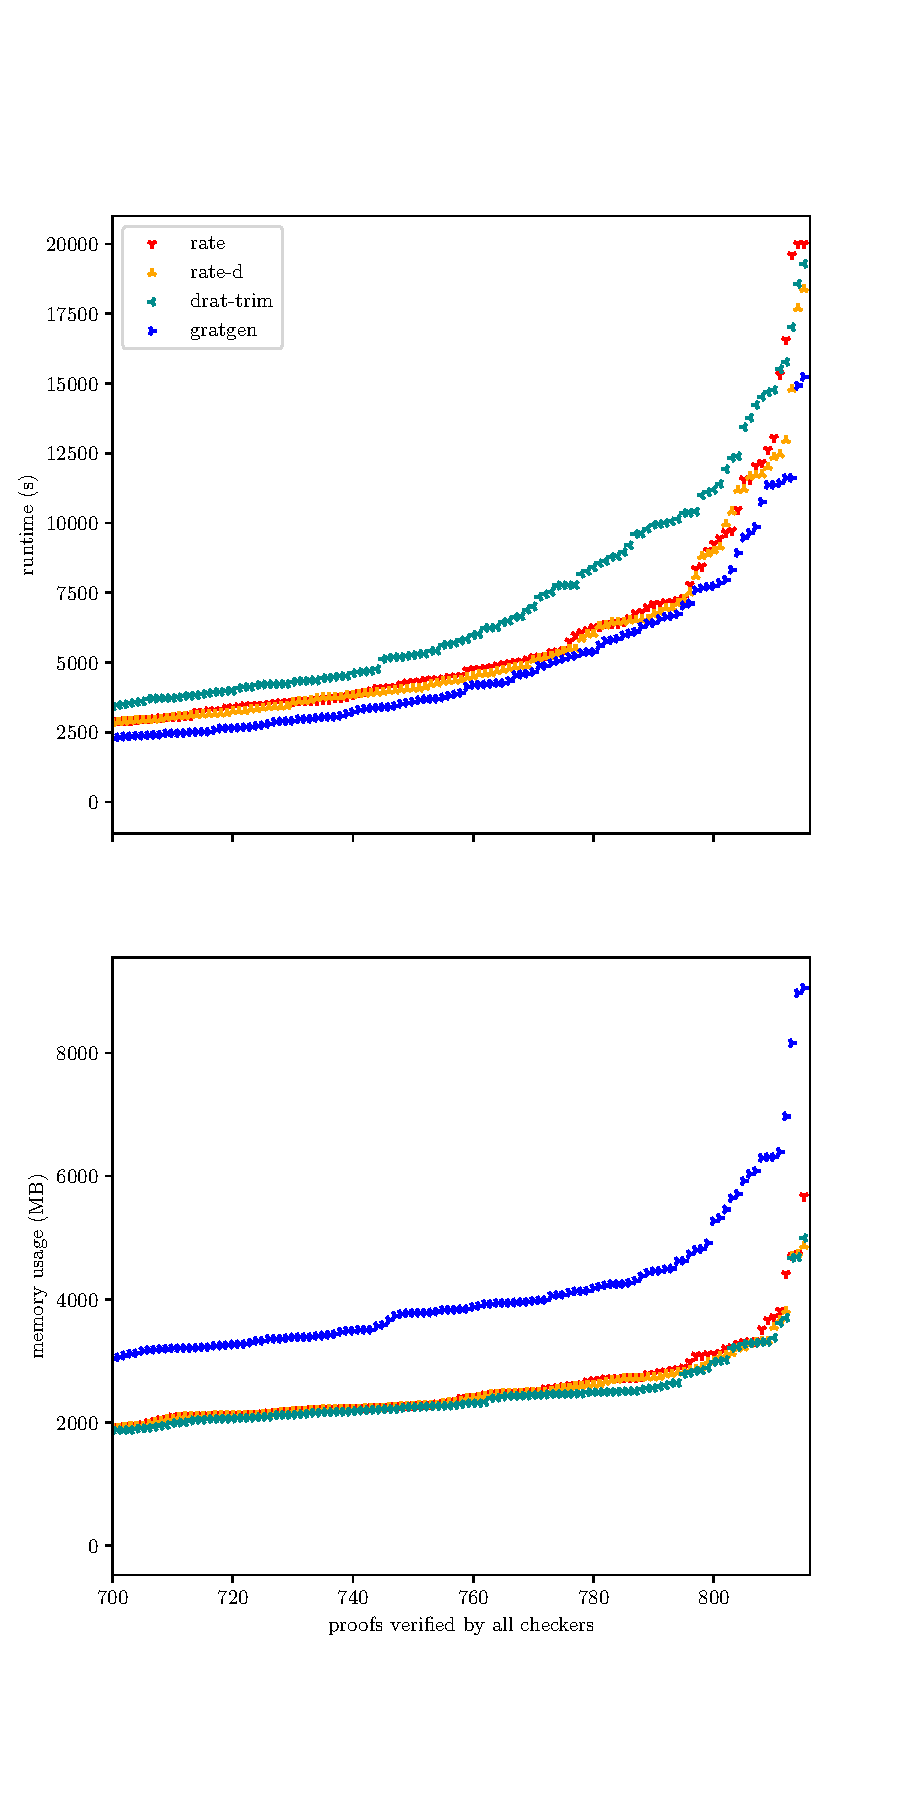
\includegraphics[width=2\textwidth,height=.9\textheight,keepaspectratio]{p/cactus.pdf}}
\caption{Cactus plot showing the distribution of checkers' runtime and memory usage.\label{fig:cactus}}
\end{figure}

\begin{figure}
% https://tex.stackexchange.com/questions/57702/custom-margin-settings-for-figure-in-latex
\centerline{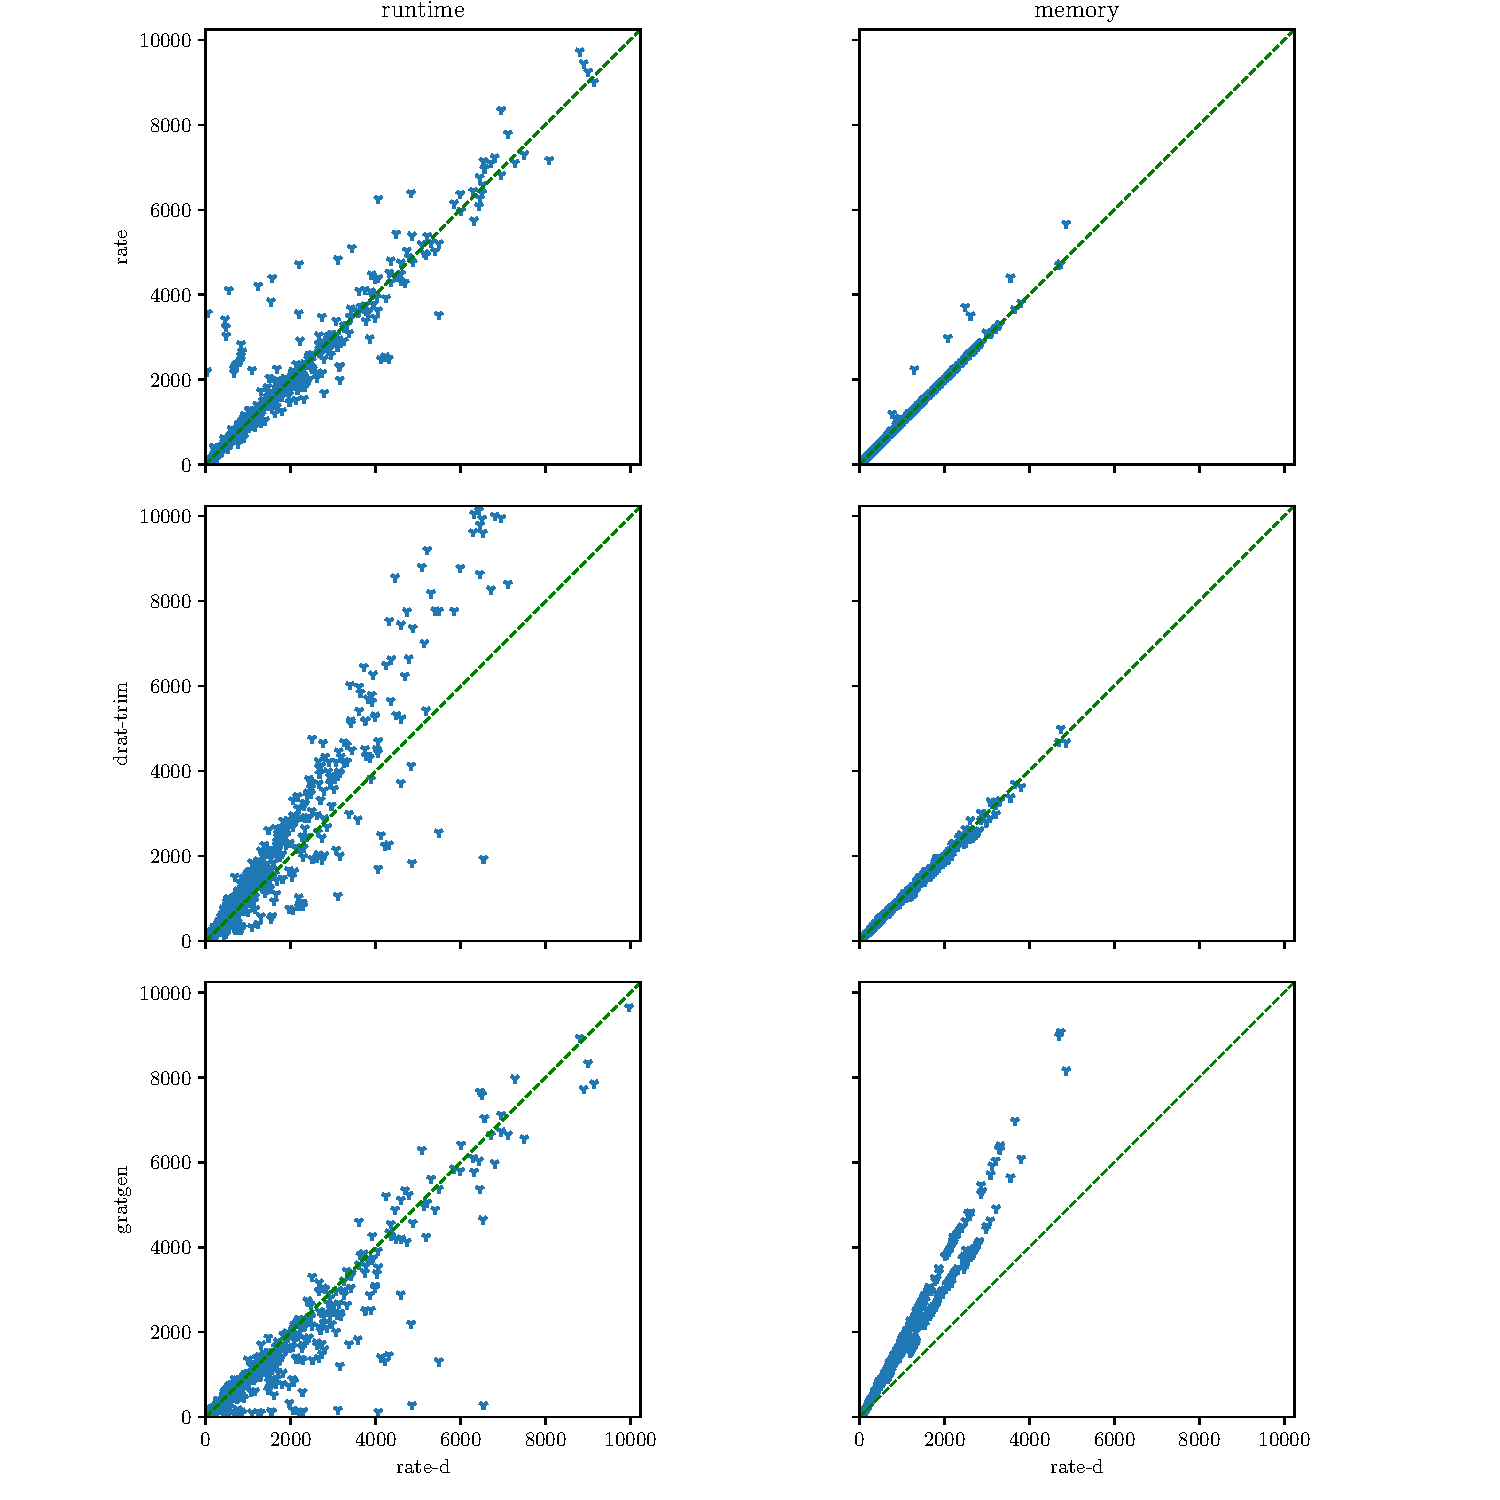
\includegraphics[width=2\textwidth,height=.9\textheight,keepaspectratio]{p/cross.pdf}}
\caption{Cross plot comparing the runtime and memory usage of
\texttt{rate\ -d} with the other checkers. Each marker represents a
proof instance.\label{fig:cross}}
\end{figure}

\hypertarget{overhead-of-reason-deletions}{%
\section{5.2 Overhead of Reason
Deletions}\label{overhead-of-reason-deletions}}

Handling reason deletions may require extra time and memory. Figure
\ref{fig:correlation-reason-deletions} shows the number of reason
deletions and the overhead of \texttt{rate} compared to \texttt{rate-d}
--- among our benchmarks runtime at most doubles. Currently,
\texttt{rate} incurs these extra costs also for proofs that contain no
unique reason deletions --- these instances are shown with red markers.

\begin{figure}
\centering
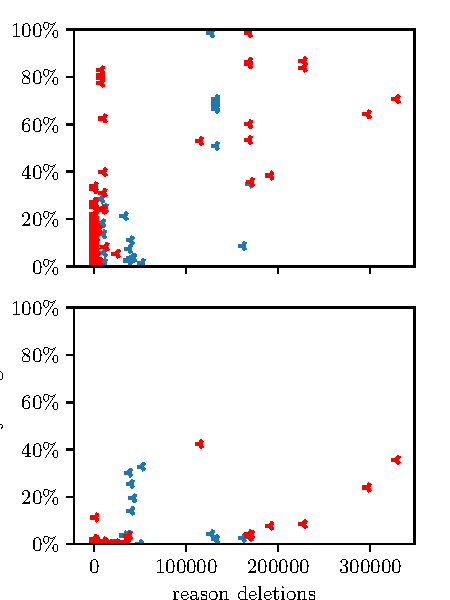
\includegraphics{p/correlation-reason-deletions.pdf}
\caption{The number of reason deletions compared to the runtime and
memory overhead of checking specified DRAT over operational
DRAT.\label{fig:correlation-reason-deletions}}
\end{figure}

\hypertarget{conclusion}{%
\chapter{6. Conclusion}\label{conclusion}}

State-of-the-art SAT solvers produce proofs with deletions of unique
reason clauses. These proofs are often incorrect under specified DRAT.
Under operational DRAT they are correct because those deletions will
effectively be removed from the proof. In
\protect\hyperlink{drat-proofs-without-deletions-of-unique-reason-clauses}{Section
3} we have explained how \texttt{DRUPMiniSat}-based solvers produce
proofs with reason deletions and we have proposed patches to avoid them,
removing the need to ignore some deletions to verify their proofs.

As we explained at the end of \protect\hyperlink{preliminaries}{Section
2}, specified DRAT is necessary to verify solvers' inprocessing steps
that employ deletions of unique reason clauses
{[}\protect\hyperlink{ref-DBLP:confux2fsatux2fRebola-PardoB18}{4}{]}.
Our initial research question was whether specified DRAT can be checked
as efficiently as operational DRAT. Previous work has yielded an
efficient algorithm but no competitive checker. We have implemented the
first checker delivering state-of-the-art performance while supporting
both specified and operational DRAT. We provide experimental results
suggesting that that the cost for specified DRAT is, on average, the
same but a high number of reason deletions may make it significantly
more costly.

The two-watched literal scheme is difficult to implement correctly, and
efficient algorithm to check specified DRAT further complicates that.
Our checker implementation is able to output LRAT and GRAT certificates
that can be verified by a formally verified checker, giving some
confidence that \texttt{rate} gave the right answer. However, many
proofs are rejected by \texttt{rate}. We needed a way to trust those
incorrectness results. We extended the previously unpublished SICK
format for proof incorrectness certificates and implemented a tool,
\texttt{sick-check} that verifies those certificates, independent of
\texttt{rate} and also much simpler than \texttt{rate}:
\texttt{sick-check} merely computes the accumulated formula up to the
failed proof step and then checks that step without doing propagation.
These certificates can be used to detect bugs in checkers (we did find
some in \texttt{rate}) and pinpoint bugs in solvers.

\hypertarget{future-work}{%
\chapter{7. Future Work}\label{future-work}}

If specified DRAT were to be adopted, it might be beneficial to
implement a way to perform deletions of non-unique reasons more
efficiently than \texttt{rate} does. These deletions do not alter the
shared UP-model but \texttt{rate} assumes they do and does more work
than necessary, which sometimes even doubles the runtime for our
benchmarks, as we showed in Figure
\ref{fig:correlation-reason-deletions}. An optimization could consist of
an efficiently computable criterion to determine if some reason clause
is unique. A simple criterion is as follows: if a reason clause for some
literal \(l\) is deleted, check if unit clause \(l\) is in the formula.
If it is, then the deleted reason is not unique and the shared UP-model
will definitely not change. This criterion might be sufficient for the
proofs produced by the second variant of the patches from
\protect\hyperlink{drat-proofs-without-deletions-of-unique-reason-clauses}{section
3}.

State-of-the-art DRAT checkers are heavily optimized for speed but they
keep the entire input proof and the resulting LRAT proof in memory. If
the available memory is at premium, some changes could be made to do
backwards checking in an online fashion, processing one proof step at a
time. Similarly, an LRAT proof line could be written to disk immediately
checking a corresponding lemma, with some postprocessing to fix the
clause IDs.

It might be possible to forego DRAT completely and directly generate
LRAT in a solver which is already done by \texttt{varisat}. This removes
the need for a complex checker at the cost of a larger proof artifact.

\hypertarget{references}{%
\chapter*{References}\label{references}}
\addcontentsline{toc}{chapter}{References}

\hypertarget{refs}{}
\leavevmode\hypertarget{ref-BrummayerBiere-SMT09}{}%
{[}1{]} R. Brummayer and A. Biere, ``Fuzzing and delta-debugging SMT
solvers,'' \emph{ACM International Conference Proceeding Series}, pp.
1--5, Jan. 2009.

\leavevmode\hypertarget{ref-DBLP:confux2fsatux2fBrummayerLB10}{}%
{[}2{]} R. Brummayer, F. Lonsing, and A. Biere, ``Automated testing and
debugging of SAT and QBF solvers,'' in \emph{Theory and applications of
satisfiability testing - SAT 2010, 13th international conference, SAT
2010, edinburgh, uk, july 11-14, 2010. Proceedings}, 2010, vol. 6175,
pp. 44--57.

\leavevmode\hypertarget{ref-DBLP:journalsux2fstvrux2fHeuleHW14}{}%
{[}3{]} M. Heule, W. A. H. Jr., and N. Wetzler, ``Bridging the gap
between easy generation and efficient verification of unsatisfiability
proofs,'' \emph{Softw. Test., Verif. Reliab.}, vol. 24, no. 8, pp.
593--607, 2014.

\leavevmode\hypertarget{ref-DBLP:confux2fsatux2fRebola-PardoB18}{}%
{[}4{]} A. Rebola-Pardo and A. Biere, ``Two flavors of DRAT,'' in
\emph{Proceedings of pragmatics of SAT 2015, austin, texas, usa,
september 23, 2015 / pragmatics of SAT 2018, oxford, uk, july 7, 2018.},
2018, vol. 59, pp. 94--110.

\leavevmode\hypertarget{ref-DBLP:confux2faaaiux2fHeule18}{}%
{[}5{]} M. J. H. Heule, ``Schur number five,'' in \emph{Proceedings of
the thirty-second AAAI conference on artificial intelligence, (aaai-18),
the 30th innovative applications of artificial intelligence (iaai-18),
and the 8th AAAI symposium on educational advances in artificial
intelligence (eaai-18), new orleans, louisiana, usa, february 2-7,
2018}, 2018, pp. 6598--6606.

\leavevmode\hypertarget{ref-DBLP:confux2ffmcadux2fRebola-PardoC18}{}%
{[}6{]} A. Rebola-Pardo and L. Cruz-Filipe, ``Complete and efficient
DRAT proof checking,'' in \emph{2018 formal methods in computer aided
design, FMCAD 2018, austin, tx, usa, october 30 - november 2, 2018},
2018, pp. 1--9.

\leavevmode\hypertarget{ref-769433}{}%
{[}7{]} J. P. Marques-Silva and K. A. Sakallah, ``GRASP: A search
algorithm for propositional satisfiability,'' \emph{IEEE Transactions on
Computers}, vol. 48, no. 5, pp. 506--521, May 1999.

\leavevmode\hypertarget{ref-DBLP:confux2fdacux2fMoskewiczMZZM01}{}%
{[}8{]} M. W. Moskewicz, C. F. Madigan, Y. Zhao, L. Zhang, and S. Malik,
``Chaff: Engineering an efficient SAT solver,'' in \emph{Proceedings of
the 38th design automation conference, DAC 2001, las vegas, nv, usa,
june 18-22, 2001}, 2001, pp. 530--535.

\leavevmode\hypertarget{ref-DBLP:seriesux2ffaiaux2fSilvaLM09}{}%
{[}9{]} J. P. M. Silva, I. Lynce, and S. Malik, ``Conflict-driven clause
learning SAT solvers,'' in \emph{Handbook of satisfiability}, vol. 185,
A. Biere, M. Heule, H. van Maaren, and T. Walsh, Eds. IOS Press, 2009,
pp. 131--153.

\leavevmode\hypertarget{ref-DBLP:confux2fcadeux2fHeuleKB17}{}%
{[}10{]} M. J. H. Heule, B. Kiesl, and A. Biere, ``Short proofs without
new variables,'' in \emph{Automated deduction - CADE 26 - 26th
international conference on automated deduction, gothenburg, sweden,
august 6-11, 2017, proceedings}, 2017, vol. 10395, pp. 130--147.

\leavevmode\hypertarget{ref-DBLP:confux2fdateux2fGoldbergN03}{}%
{[}11{]} E. I. Goldberg and Y. Novikov, ``Verification of proofs of
unsatisfiability for CNF formulas,'' in \emph{2003 design, automation
and test in europe conference and exposition (DATE 2003), 3-7 march
2003, munich, germany}, 2003, pp. 10886--10891.

\leavevmode\hypertarget{ref-DBLP:confux2fisaimux2fGelder08}{}%
{[}12{]} A. V. Gelder, ``Verifying RUP proofs of propositional
unsatisfiability,'' in \emph{International symposium on artificial
intelligence and mathematics, ISAIM 2008, fort lauderdale, florida, usa,
january 2-4, 2008}, 2008.

\leavevmode\hypertarget{ref-DBLP:confux2fcadeux2fJarvisaloHB12}{}%
{[}13{]} M. Järvisalo, M. Heule, and A. Biere, ``Inprocessing rules,''
in \emph{Automated reasoning - 6th international joint conference, IJCAR
2012, manchester, uk, june 26-29, 2012. Proceedings}, 2012, vol. 7364,
pp. 355--370.

\leavevmode\hypertarget{ref-DBLP:confux2fcadeux2fHeuleHW13}{}%
{[}14{]} M. Heule, W. A. H. Jr., and N. Wetzler, ``Verifying refutations
with extended resolution,'' in \emph{Automated deduction - CADE-24 -
24th international conference on automated deduction, lake placid, ny,
usa, june 9-14, 2013. Proceedings}, 2013, vol. 7898, pp. 345--359.

\leavevmode\hypertarget{ref-DBLP:journalsux2famaiux2fGelder12}{}%
{[}15{]} A. V. Gelder, ``Producing and verifying extremely large
propositional refutations - have your cake and eat it too,'' \emph{Ann.
Math. Artif. Intell.}, vol. 65, no. 4, pp. 329--372, 2012.

\leavevmode\hypertarget{ref-DBLP:confux2fsatux2fWetzlerHH14}{}%
{[}16{]} N. Wetzler, M. Heule, and W. A. H. Jr., ``DRAT-trim: Efficient
checking and trimming using expressive clausal proofs,'' in \emph{Theory
and applications of satisfiability testing - SAT 2014 - 17th
international conference, held as part of the vienna summer of logic,
VSL 2014, vienna, austria, july 14-17, 2014. Proceedings}, 2014, vol.
8561, pp. 422--429.

\leavevmode\hypertarget{ref-DBLP:journalsux2fcorrux2fHeule16}{}%
{[}17{]} M. J. H. Heule, ``The DRAT format and drat-trim checker,''
\emph{CoRR}, vol. abs/1610.06229, 2016.

\leavevmode\hypertarget{ref-DBLP:confux2flparux2fPhilippR17}{}%
{[}18{]} T. Philipp and A. Rebola-Pardo, ``Towards a semantics of
unsatisfiability proofs with inprocessing,'' in \emph{LPAR-21, 21st
international conference on logic for programming, artificial
intelligence and reasoning, maun, botswana, may 7-12, 2017}, 2017, vol.
46, pp. 65--84.

\leavevmode\hypertarget{ref-DBLP:confux2fcadeux2fCruz-FilipeHHKS17}{}%
{[}19{]} L. Cruz-Filipe, M. J. H. Heule, W. A. H. Jr., M. Kaufmann, and
P. Schneider-Kamp, ``Efficient certified RAT verification,'' in
\emph{Automated deduction - CADE 26 - 26th international conference on
automated deduction, gothenburg, sweden, august 6-11, 2017,
proceedings}, 2017, vol. 10395, pp. 220--236.

\leavevmode\hypertarget{ref-DBLP:confux2fitpux2fHeuleHKW17}{}%
{[}20{]} M. Heule, W. A. H. Jr., M. Kaufmann, and N. Wetzler,
``Efficient, verified checking of propositional proofs,'' in
\emph{Interactive theorem proving - 8th international conference, ITP
2017, brasilia, brazil, september 26-29, 2017, proceedings}, 2017, vol.
10499, pp. 269--284.

\leavevmode\hypertarget{ref-DBLP:confux2ffmcadux2fHeuleHW13}{}%
{[}21{]} M. Heule, W. A. H. Jr., and N. Wetzler, ``Trimming while
checking clausal proofs,'' in \emph{Formal methods in computer-aided
design, FMCAD 2013, portland, or, usa, october 20-23, 2013}, 2013, pp.
181--188.

\leavevmode\hypertarget{ref-DBLP:confux2fjeliaux2fPhilippR16}{}%
{[}22{]} T. Philipp and A. Rebola-Pardo, ``DRAT proofs for XOR
reasoning,'' in \emph{Logics in artificial intelligence - 15th european
conference, JELIA 2016, larnaca, cyprus, november 9-11, 2016,
proceedings}, 2016, vol. 10021, pp. 415--429.

\leavevmode\hypertarget{ref-DBLP:confux2fcadeux2fHeuleHW15}{}%
{[}23{]} M. Heule, W. A. H. Jr., and N. Wetzler, ``Expressing symmetry
breaking in DRAT proofs,'' in \emph{Automated deduction - CADE-25 - 25th
international conference on automated deduction, berlin, germany, august
1-7, 2015, proceedings}, 2015, vol. 9195, pp. 591--606.

\leavevmode\hypertarget{ref-DBLP:confux2fsatux2fLammich17}{}%
{[}24{]} P. Lammich, ``The GRAT tool chain - efficient (UN)SAT
certificate checking with formal correctness guarantees,'' in
\emph{Theory and applications of satisfiability testing - SAT 2017 -
20th international conference, melbourne, vic, australia, august 28 -
september 1, 2017, proceedings}, 2017, vol. 10491, pp. 457--463.

\leavevmode\hypertarget{ref-DBLP:confux2fcadeux2fLammich17}{}%
{[}25{]} P. Lammich, ``Efficient verified (UN)SAT certificate
checking,'' in \emph{Automated deduction - CADE 26 - 26th international
conference on automated deduction, gothenburg, sweden, august 6-11,
2017, proceedings}, 2017, vol. 10395, pp. 237--254.

\leavevmode\hypertarget{ref-Tange2018}{}%
{[}26{]} O. Tange, \emph{GNU parallel 2018}. Ole Tange, 2018.

\end{document}
